\documentclass[tikz,border=2pt]{standalone}
\usepackage[T1]{fontenc}
\usepackage{lmodern}
\usepackage{amsmath,amssymb}
\usepackage{enumitem}
\usepackage[dvipsnames]{xcolor}
\usetikzlibrary{arrows.meta}
% Compact, readable defaults; theorem Markdown can override these per list.
\setlist[itemize,1]{
  leftmargin=1.35em,
  topsep=2pt plus 1pt minus 1pt,
  parsep=0pt,
  itemsep=1pt plus .5pt,
  partopsep=0pt
}

\begin{document}
% Generated from companion_to_analysis_ch_1_to_3_graph.md by theorem-dependency-graph.
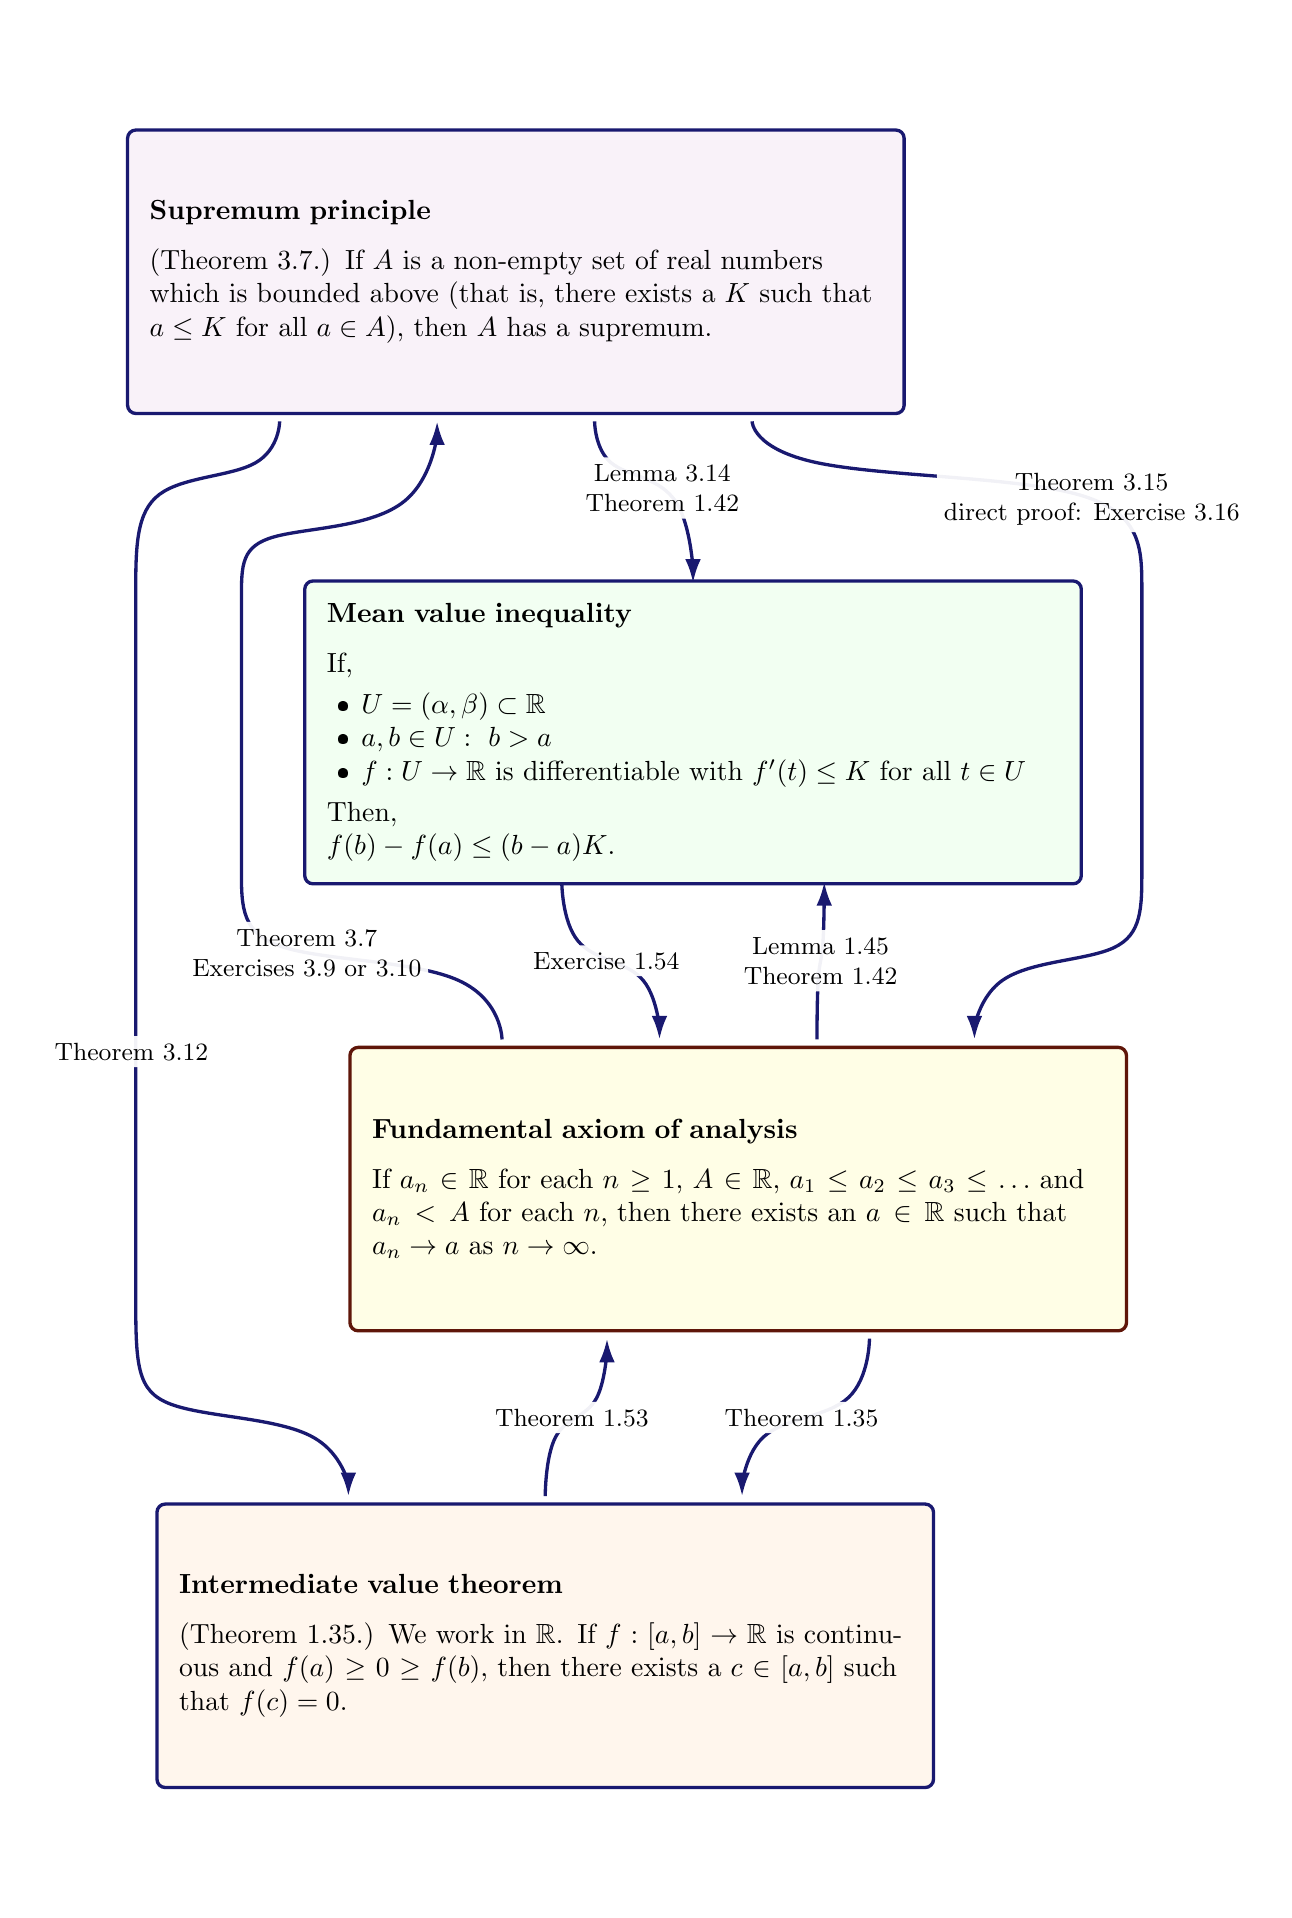
\begin{tikzpicture}[x=1cm, y=1cm, >=Latex]
    \path[use as bounding box] (-7.692638893333334,-11.824999999027778) rectangle (8.010783305355188,11.824999999027778);
    \draw[-{Latex[length=3mm,width=2mm]}, very thick, draw=MidnightBlue] (-1.668611,-1.025000) .. controls (-1.668611,-1.025000) and (-1.668611,-0.525000) .. (-2.220162,-0.275000) .. controls (-2.771713,-0.025000) and (-3.874815,-0.025000) .. (-4.426366,0.141667) .. controls (-4.977917,0.308333) and (-4.977917,0.641667) .. (-4.977917,1.125000) .. controls (-4.977917,1.608333) and (-4.977917,2.241667) .. (-4.977917,2.875000) .. controls (-4.977917,3.508333) and (-4.977917,4.141667) .. (-4.977917,4.575000) .. controls (-4.977917,5.008333) and (-4.977917,5.241667) .. (-4.563704,5.358333) .. controls (-4.149491,5.475000) and (-3.321065,5.475000) .. (-2.906852,5.812500) .. controls (-2.492639,6.150000) and (-2.492639,6.825000) .. (-2.492639,6.825000);
    \node[fill=white, fill opacity=0.94, text opacity=1, rounded corners=2pt, inner sep=2.5pt, align=center, font=\small] at (-4.148020979982553, 0.07716838068990485) { Theorem 3.7\\Exercises 3.9 or 3.10 };
    \draw[-{Latex[length=3mm,width=2mm]}, very thick, draw=MidnightBlue] (1.507361,6.825000) .. controls (1.507361,6.825000) and (1.507361,6.475000) .. (2.332361,6.300000) .. controls (3.157361,6.125000) and (4.807361,6.125000) .. (5.632361,5.900000) .. controls (6.457361,5.675000) and (6.457361,5.225000) .. (6.457361,4.683333) .. controls (6.457361,4.141667) and (6.457361,3.508333) .. (6.457361,2.875000) .. controls (6.457361,2.241667) and (6.457361,1.608333) .. (6.457361,1.125000) .. controls (6.457361,0.641667) and (6.457361,0.308333) .. (6.103032,0.141667) .. controls (5.748704,-0.025000) and (5.040046,-0.025000) .. (4.685718,-0.275000) .. controls (4.331389,-0.525000) and (4.331389,-1.025000) .. (4.331389,-1.025000);
    \node[fill=white, fill opacity=0.94, text opacity=1, rounded corners=2pt, inner sep=2.5pt, align=center, font=\small] at (5.820783305355188, 5.838727009755482) { Theorem 3.15\\direct proof: Exercise 3.16 };
    \draw[-{Latex[length=3mm,width=2mm]}, very thick, draw=MidnightBlue] (2.331389,-1.025000) .. controls (2.331389,-1.025000) and (2.331389,-0.525000) .. (2.346829,-0.275000) .. controls (2.362269,-0.025000) and (2.393148,-0.025000) .. (2.408588,0.225000) .. controls (2.424028,0.475000) and (2.424028,0.975000) .. (2.424028,0.975000);
    \node[fill=white, fill opacity=0.94, text opacity=1, rounded corners=2pt, inner sep=2.5pt, align=center, font=\small] at (2.3777083264583307, -0.025000020555555516) { Lemma 1.45\\Theorem 1.42 };
    \draw[-{Latex[length=3mm,width=2mm]}, very thick, draw=MidnightBlue] (-0.909306,0.975000) .. controls (-0.909306,0.975000) and (-0.909306,0.475000) .. (-0.702523,0.225000) .. controls (-0.495741,-0.025000) and (-0.082176,-0.025000) .. (0.124606,-0.275000) .. controls (0.331389,-0.525000) and (0.331389,-1.025000) .. (0.331389,-1.025000);
    \node[fill=white, fill opacity=0.94, text opacity=1, rounded corners=2pt, inner sep=2.5pt, align=center, font=\small] at (-0.28895834020833283, -0.025000020555554354) { Exercise 1.54 };
    \draw[-{Latex[length=3mm,width=2mm]}, very thick, draw=MidnightBlue] (2.998056,-4.825000) .. controls (2.998056,-4.825000) and (2.998056,-5.325000) .. (2.728449,-5.575000) .. controls (2.458843,-5.825000) and (1.919630,-5.825000) .. (1.650023,-6.075000) .. controls (1.380417,-6.325000) and (1.380417,-6.825000) .. (1.380417,-6.825000);
    \node[fill=white, fill opacity=0.94, text opacity=1, rounded corners=2pt, inner sep=2.5pt, align=center, font=\small] at (2.1892361001388854, -5.8250000069444425) { Theorem 1.35 };
    \draw[-{Latex[length=3mm,width=2mm]}, very thick, draw=MidnightBlue] (-1.119583,-6.825000) .. controls (-1.119583,-6.825000) and (-1.119583,-6.325000) .. (-0.988866,-6.075000) .. controls (-0.858148,-5.825000) and (-0.596713,-5.825000) .. (-0.465995,-5.575000) .. controls (-0.335278,-5.325000) and (-0.335278,-4.825000) .. (-0.335278,-4.825000);
    \node[fill=white, fill opacity=0.94, text opacity=1, rounded corners=2pt, inner sep=2.5pt, align=center, font=\small] at (-0.7274305665277802, -5.8250000069444425) { Theorem 1.53 };
    \draw[-{Latex[length=3mm,width=2mm]}, very thick, draw=MidnightBlue] (-4.492639,6.825000) .. controls (-4.492639,6.825000) and (-4.492639,6.475000) .. (-4.797292,6.300000) .. controls (-5.101944,6.125000) and (-5.711250,6.125000) .. (-6.015903,5.900000) .. controls (-6.320556,5.675000) and (-6.320556,5.225000) .. (-6.320556,4.600000) .. controls (-6.320556,3.975000) and (-6.320556,3.175000) .. (-6.320556,2.375000) .. controls (-6.320556,1.575000) and (-6.320556,0.775000) .. (-6.320556,-0.425000) .. controls (-6.320556,-1.625000) and (-6.320556,-3.225000) .. (-6.320556,-4.191667) .. controls (-6.320556,-5.158333) and (-6.320556,-5.491667) .. (-5.870394,-5.658333) .. controls (-5.420231,-5.825000) and (-4.519907,-5.825000) .. (-4.069745,-6.075000) .. controls (-3.619583,-6.325000) and (-3.619583,-6.825000) .. (-3.619583,-6.825000);
    \node[fill=white, fill opacity=0.94, text opacity=1, rounded corners=2pt, inner sep=2.5pt, align=center, font=\small] at (-6.320555574861115, -1.178651910113754) { Theorem 3.12 };
    \draw[-{Latex[length=3mm,width=2mm]}, very thick, draw=MidnightBlue] (-0.492639,6.825000) .. controls (-0.492639,6.825000) and (-0.492639,6.475000) .. (-0.284306,6.300000) .. controls (-0.075972,6.125000) and (0.340694,6.125000) .. (0.549028,5.787500) .. controls (0.757361,5.450000) and (0.757361,4.775000) .. (0.757361,4.775000);
    \node[fill=white, fill opacity=0.94, text opacity=1, rounded corners=2pt, inner sep=2.5pt, align=center, font=\small] at (0.3676893348790949, 5.979727245070155) { Lemma 3.14\\Theorem 1.42 };
    \node[draw=MidnightBlue, very thick, rounded corners=3pt, fill=blue!4, text width=9.3cm, minimum height=3.6cm, inner sep=8pt, align=left, font=\normalsize, fill=violet!5] at (-1.492638894444445, 8.72500000013889) { \textbf{Supremum principle}\par\medskip (Theorem 3.7.) If $A$ is a non-empty set of real numbers which is bounded above (that is, there exists a $K$ such that $a \leq K$ for all $a \in A$), then $A$ has a supremum. };
    \node[draw=MidnightBlue, very thick, rounded corners=3pt, fill=blue!4, text width=9.3cm, minimum height=3.6cm, inner sep=8pt, align=left, font=\normalsize, fill=green!5] at (0.7573611055555548, 2.8749999726388897) { \textbf{Mean value inequality}\par\medskip If,

\begin{itemize}[ noitemsep, topsep=1pt, leftmargin=1.25em, labelsep=0.4em ] \item $U = (\alpha, \beta) \subset \mathbb{R}$ \item $a,b \in U : \ b > a$ \item $f:U\to\mathbb{R}$ is differentiable with $f'(t)\leq K$ for all $t\in U$ \end{itemize}

Then,

$f(b)-f(a)\leq(b-a)K$. };
    \node[draw=MidnightBlue, very thick, rounded corners=3pt, fill=blue!4, text width=9.3cm, minimum height=3.6cm, inner sep=8pt, align=left, font=\normalsize, fill=yellow!10, draw=Sepia] at (1.3313888806944445, -2.9250000137499987) { \textbf{Fundamental axiom of analysis}\par\medskip If $a_n \in \mathbb{R}$ for each $n \geq 1$, $A \in \mathbb{R}$, $a_1 \leq a_2 \leq a_3 \leq \ldots$ and $a_n < A$ for each $n$, then there exists an $a \in \mathbb{R}$ such that $a_n \to a$ as $n \to \infty$. };
    \node[draw=MidnightBlue, very thick, rounded corners=3pt, fill=blue!4, text width=9.3cm, minimum height=3.6cm, inner sep=8pt, align=left, font=\normalsize, fill=orange!7] at (-1.1195833470833336, -8.725000000138888) { \textbf{Intermediate value theorem}\par\medskip (Theorem 1.35.) We work in $\mathbb{R}$. If $f:[a,b]\to\mathbb{R}$ is continuous and $f(a)\geq0\geq f(b)$, then there exists a $c\in[a,b]$ such that $f(c)=0$. };
\end{tikzpicture}
\end{document}
